\documentclass[table, aspectratio=169]{beamer}

\usetheme[serif, sansserifheader]{tugrazivc}
% options:
% * serif loads \lmodern and enables serifs everywhere
% * webfonst loads switches to tugraz webfonts, more corporate
% * sansserifheader removes serifs in headers and on title page
% * sectionhead adds section names in header of each slide

% use this theme if you want to get rid of the section header and use the tugraz webfont
% \usetheme[webfonts]{tugrazivc}
 
\usepackage[utf8]{inputenc}
\usepackage[english]{babel}
\usetikzlibrary{overlay-beamer-styles}

\usepackage{pgfplots} % Plots and diagrams
\usetikzlibrary{shapes,shapes.misc}
\DeclareUnicodeCharacter{2212}{−}
\usepgfplotslibrary{groupplots,dateplot}
\usetikzlibrary{patterns,shapes.arrows}
\usepackage{tabularray}  % Coloured tables -- requires [table] option for beamer
\usepackage{fontawesome} % Useful icons (\faName)
\usepackage[style=ieee, bibencoding=utf8]{biblatex} % Bibliography
\addbibresource{references.bib}
\usepackage{csquotes}
\usepackage{amsmath}
\usepackage{amssymb}
\usepackage{bm}
\usepackage{csquotes}
\usepackage{subcaption}
\usepackage{varwidth}
\usepackage{svg}
\usepackage{booktabs}
\usepackage{epigraph}

\usepackage[acronym, nomain]{glossaries}
\usefonttheme{default}
\addtobeamertemplate{frametitle}{}{\vspace*{-2em}}

\makeglossaries
\newacronym[shortplural=IAIs, longplural=interpretable artifical intelligence]{iai}{IAI}{interpretable artificial intelligence}


\addbibresource{../../literature/sources.bib}

\title[IVC Seminar SS2025]{In-Silico Cancer Cell}
\author[Peter Waldert]{\textbf{Peter Waldert}}
\date{\today}
\institute{IVC}
\instituteurl{ivc.tugraz.at}

\begin{document}
  \begin{frame}[plain]
    \maketitle
  \end{frame}

  \begin{frame}{Biological Setting: Cancer Cell}
    %% A549 model (lung cancer)
    %% with picture
    \begin{columns}
      \begin{column}{0.4\linewidth}
        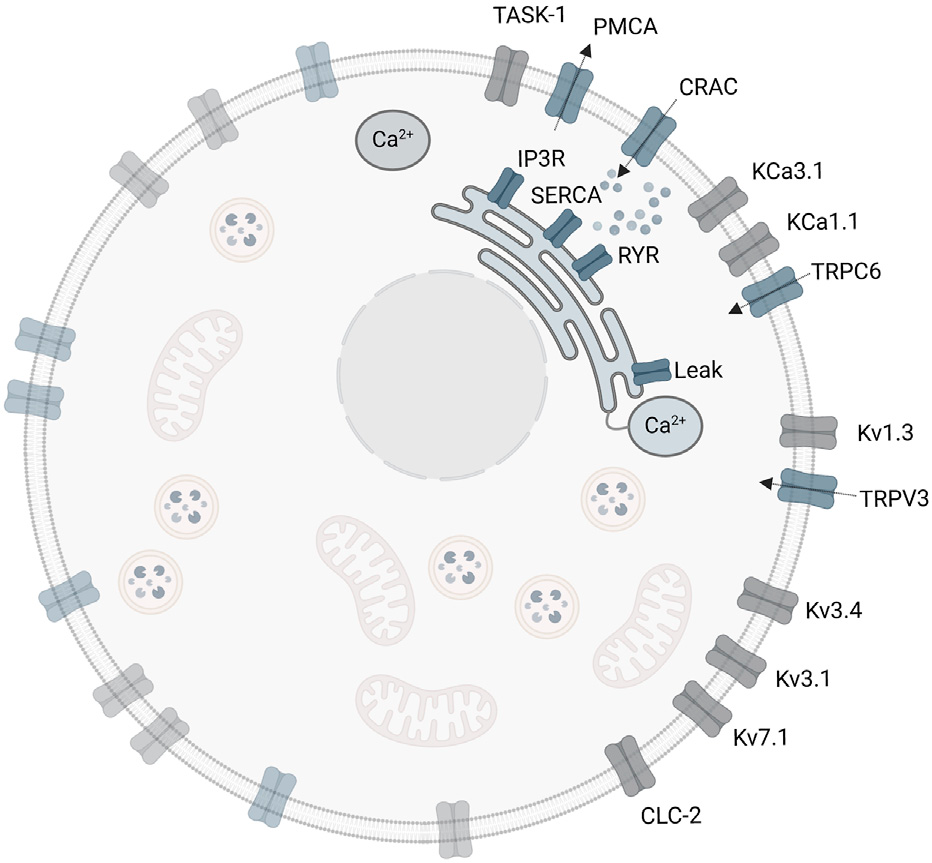
\includegraphics[width=\linewidth]{../../figures/cell-by-langthaler-et-al.png}
      \end{column}
      \begin{column}{0.58\linewidth}
        Indeed
      \end{column}
    \end{columns}
  \end{frame}

  \begin{frame}{Experiment: Patch-Clamping}
    %% describe, with picture
    %% we measure current based on voltage changes
    \begin{columns}
      \begin{column}{0.4\linewidth}
        \begin{figure}
          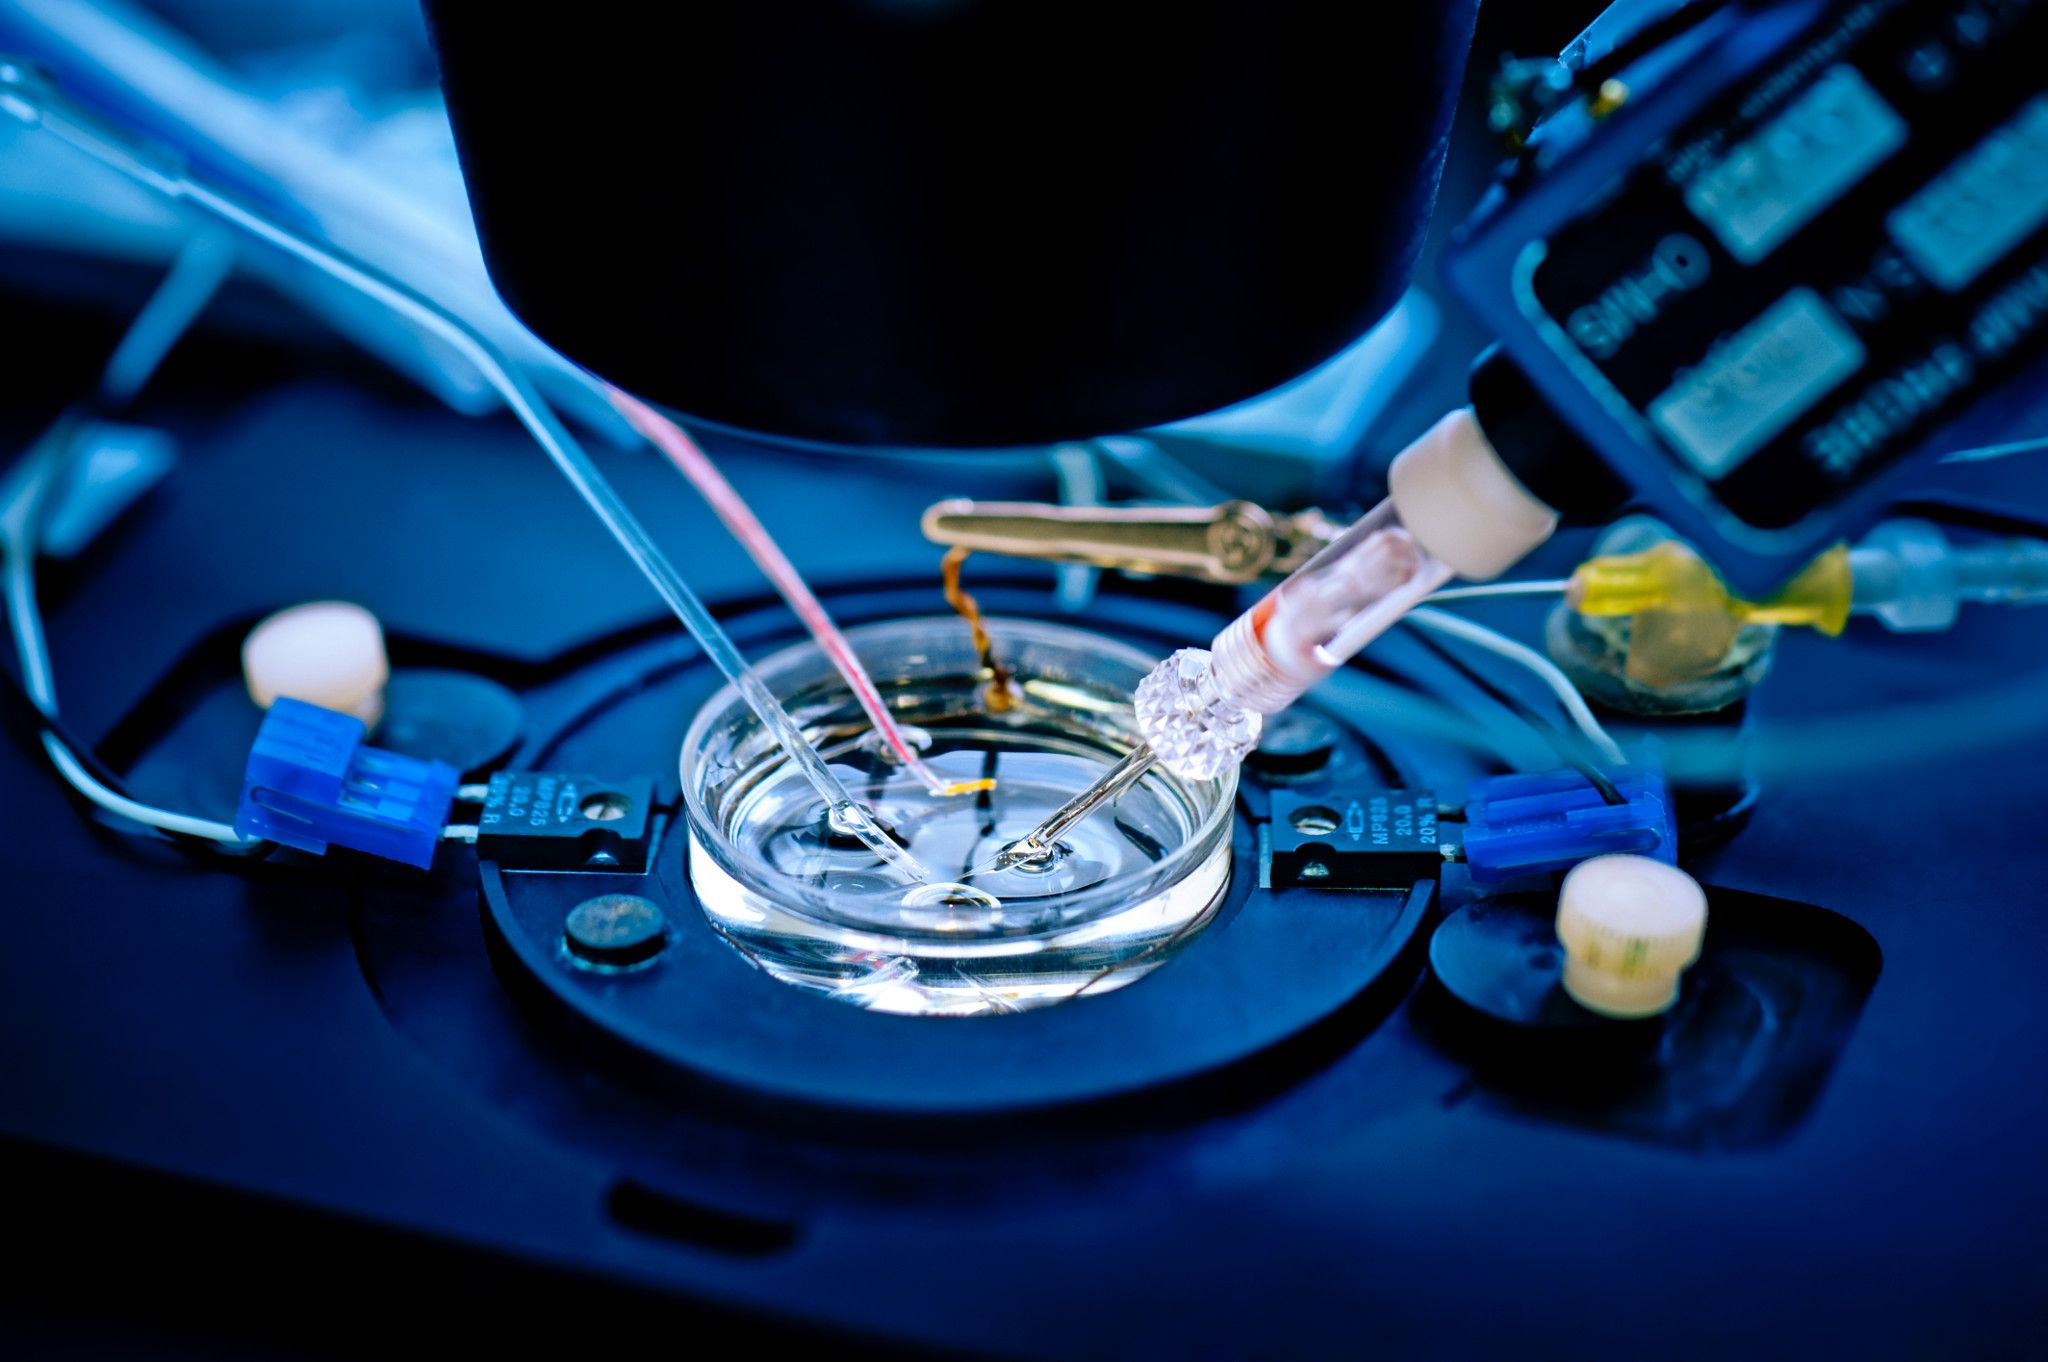
\includegraphics[width=\linewidth]{../../figures/patch-clamp-system.jpeg}
          \caption{Patch-Clamp System \cite{2025-patch-clamp-image}}
        \end{figure}
      \end{column}
      \begin{column}{0.58\linewidth}
        Approach in which electrophysiological behaviour of a cell can be measured in a lab.
        \begin{itemize}
          \item Cell-attached recording method
          \item Whole-cell recording method
        \end{itemize}
      \end{column}
    \end{columns}
  \end{frame}

  \begin{frame}{Simulation of the Experiment}
    %% Multiple independent Ion Channels
    %% Each follows: $$
  \end{frame}

  \begin{frame}{Hidden Markov Model}
    %% very nice, describe transition matrix and dependence on V, t

  \end{frame}

  \begin{frame}{Solution of the Inverse Problem}
    %% using different methods, based on LSQ.
    %% reformulation into a quadratic problem
  \end{frame}

  \begin{frame}{Runtime Optimisation}
    %% using adaptive timestepping

  \end{frame}

  \begin{frame}{Visualisation Dashboard}
    %% Based on Astro and @observablehq/plot, but mostly:

  \end{frame}
  \begin{frame}{WebAssembly}
    %% Compilation of Rust code
    %% Solver: [insert]
  \end{frame}

  \section{Simulation}
  \begin{frame}{Cancer Cell Simulation}
    \begin{itemize}
      \item Let's go!
    \end{itemize}
  \end{frame}

  \begin{frame}[allowframebreaks]{References}
    \printbibliography
  \end{frame}
\end{document}
